\subsection{Izračun krivulj}
Za vsako krivuljo sem izračunal, kakšna naj bi bila glede na
željene parametre, nato sem poiskal, ali jo ima že kakšno podobno
podjetje, v nasprotnem primeru jo bom izdelal sam.
Čas enega cikla, tj. enkraten obrat krivuljne gredi, bo 10 s.
Formule sem uporabil iz poglavja \nameref{izracun_krivulj}

\subsubsection{Struženje roba}
Vrtljaji: 2000 \( \frac{vrt}{min} \) \\
Pomik: 0,04 \( \frac{mm}{vrt} \) \\
Dolžina struženja: 1 mm

Z zgornjimi podatki izračunamo potreben čas:
\begin{equation}
	\begin{split}
		t &= \frac{l*60\ s}{f*S} \\
		t &= \frac{1\ mm*60\ s}{0,04\ \frac{mm}{obr}*2000\ \frac{obr}{min}} \\
		t &= 0,75\ s,
	\end{split}
\end{equation}
nato pa še kot vzpona krivulje:
\begin{equation}
	\begin{split}
		\alpha &= \frac{360\degree}{T} * t \\
		\alpha &= \frac{360\degree}{10\ s} * 0,75\ s\\
		\alpha &= 27\degree.
	\end{split}
\end{equation}

Spodaj na Sliki \ref{shema_robov} sem narisal še skico orodja
in obdelovanca pri pobiranju robov.
\begin{figure}[H]
	\begin{center}
		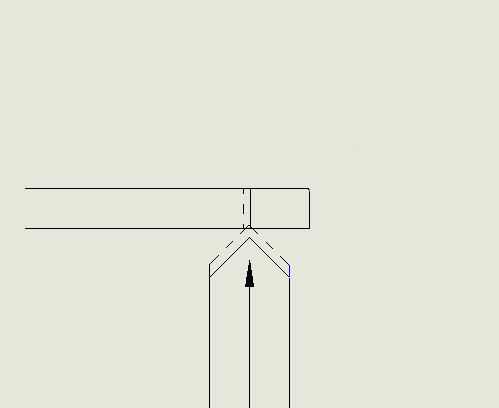
\includegraphics[width=8cm]{robi.png}
		\caption{Skica poteka pobiranja robov
			\cite{lasten}}
		\label{shema_robov}
	\end{center}
\end{figure}

\subsubsection{Središčenje}
Vrtljaji: 2000 \( \frac{vrt}{min} \) + 2200 \( \frac{vrt}{min} \)\\
Pomik: 0,03 \( \frac{mm}{vrt} \) \\
Dolžina vrtanja: 2 mm

Enako krivuljo sem uporabil tudi za povrtavanje luknje z druge strani.
\begin{equation}
	\begin{split}
		t &= \frac{l*60\ s}{f*S} \\
		t &= \frac{2\ mm*60\ s}{0,03\ \frac{mm}{obr}*4200\ \frac{obr}{min}} \\
		t &= 0,95\ s
	\end{split}
\end{equation}
\begin{equation}
	\begin{split}
		\alpha &= \frac{360\degree}{T} * t \\
		\alpha &= \frac{360\degree}{10\ s} * 0,95\  s\\
		\alpha &= 34,2\degree
	\end{split}
\end{equation}
Spodaj na Sliki \ref{centriranje} je prikazan potek
centriranja pred vrtanjem.
\begin{figure}[H]
	\begin{center}
		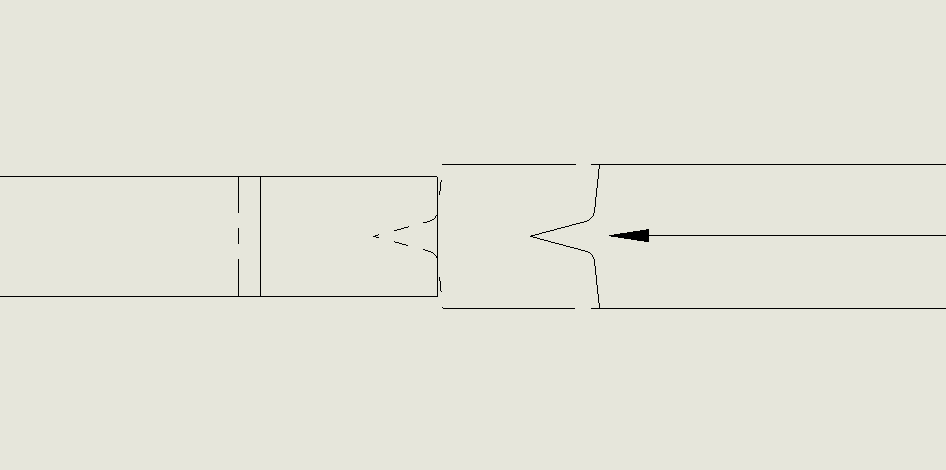
\includegraphics[width=8cm]{centriranje.png}
		\caption{Skica poteka centriranja
			\cite{lasten}}
		\label{centriranje}
	\end{center}
\end{figure}
\subsubsection{Vrtanje}
Vrtljaji: 2000 \( \frac{vrt}{min} \) + 2200 \( \frac{vrt}{min} \)\\
Pomik: 0,03 \( \frac{mm}{vrt} \) \\
Dolžina vrtanja: 8 mm
\begin{equation}
	\begin{split}
		t &= \frac{l*60\ s}{f*S} \\
		t &= \frac{8\ mm*60\ s}{0,03\ \frac{mm}{obr}*4200\ \frac{obr}{min}} \\
		t &= 3,8\ s
	\end{split}
\end{equation}
\begin{equation}
	\begin{split}
		\alpha &= \frac{360\degree}{T} * t \\
		\alpha &= \frac{360\degree}{10\ s} * 3,8\ s\\
		\alpha &= 136,8\degree
	\end{split}
\end{equation}
Na spodnji Sliki \ref{vrtanje} je prikazana skica vrtanja
luknje $\phi 1,4$.
\begin{figure}[H]
	\begin{center}
		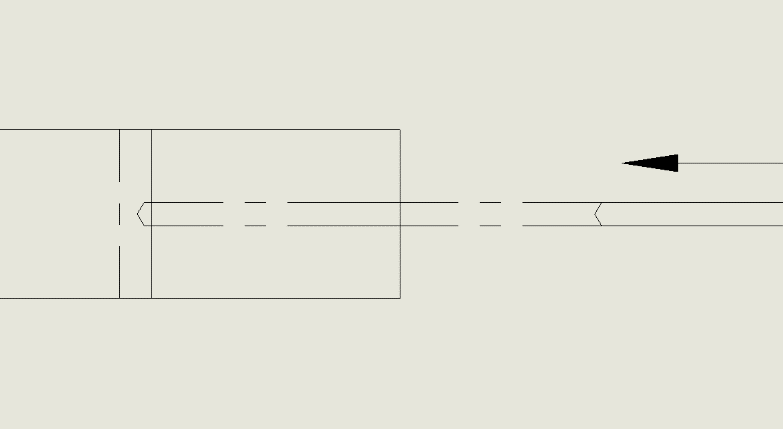
\includegraphics[width=8cm]{vrtanje.png}
		\caption{Skica poteka vrtanja
			\cite{lasten}}
		\label{vrtanje}
	\end{center}
\end{figure}
Zaradi večje globine vrtanja in malega premera svedra
sem v krivuljo dodal luknjo zato, ker se navadno vrta globino, ki znaša trikratnik
premera svedra v eni potezi, za globje luknje pa se sveder
izvleče, da se ohladi in očisti ostružkov, nakar se nadaljuje vrtanje.
Za premik svedrov se na tem stroju uporablja bobnaste krivulje,
zato sem skiciral raztegnjeno bobnasto krvuljo, kot je prikazano
na Sliki \ref{raztegnjen_boben}.
\begin{figure}[H]
	\begin{center}
		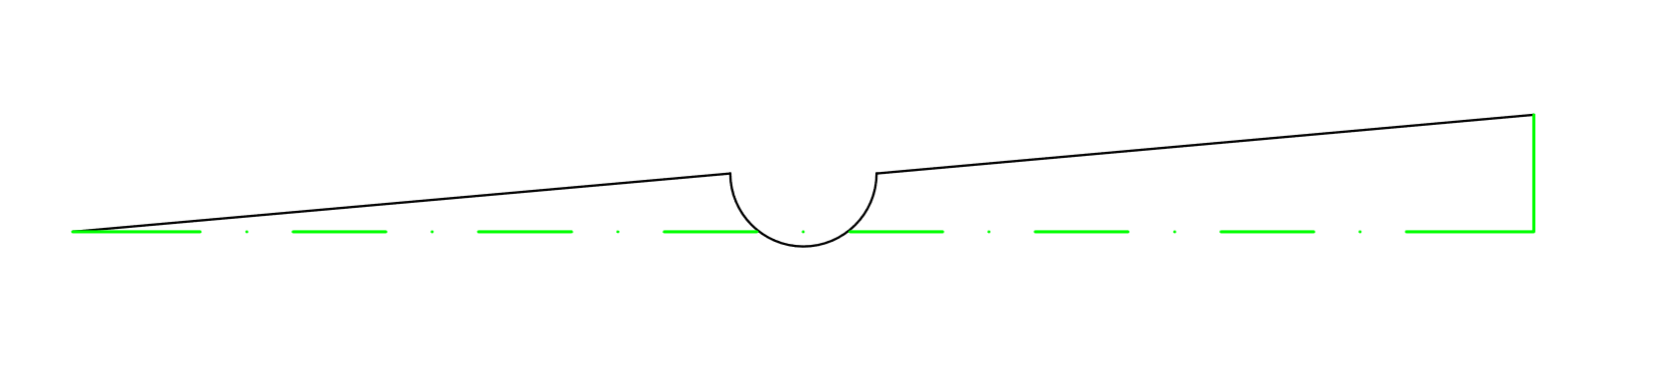
\includegraphics[width=\linewidth]{skica_krivulje_vrtanja.png}
		\caption{Raztegnjena bobnasta krivulja
			\cite{lasten}}
		\label{raztegnjen_boben}
	\end{center}
\end{figure}
\subsubsection{Odrez}
\label{izracun_odreza}
Vrtljaji: 2000 \( \frac{vrt}{min} \) \\
Pomik: 0,02 \( \frac{mm}{vrt} \) \\
Dolžina struženja: 3 mm
\begin{equation}
	\begin{split}
		t &= \frac{l*60\ s}{f*S} \\
		t &= \frac{3\ mm*60\ s}{0,02\ \frac{mm}{obr}*2000\ \frac{obr}{min}} \\
		t &= 4,5\ s
	\end{split}
\end{equation}
\begin{equation}
	\begin{split}
		\alpha &= \frac{360\degree}{T} * t \\
		\alpha &= \frac{360\degree}{10\ s} * 3,8\ s\\
		\alpha &= 146\degree
	\end{split}
\end{equation}

\subsubsection{Rezultati izračunov in izbira standardnih krivulj}
V spodnji Tabeli \ref{Tabela rezultatov} so prikazani
rezultati mojih izračunov, s katerimi sem izbral približno
enake standardne krivulje, ki jih je imelo podjetje na zalogi.
Zato da se sledilci manj obrabljajo in da se zmanjša sila sledilca
na krivuljo, sem se odločil za vse krivulje uporabiti razmerje ročic
5:1, kar pomeni, da se bo za 5 mm vzpona krivulje orodje premaknilo za 1 mm.

\begin{table}[H]
	\caption{Povzetki izračunov krivulj}
	\label{Tabela rezultatov}
	\begin{center}
		\begin{tabular}{|c|c|c|c|c|}
			\hline
			Operacija      & Vzpon [mm] & Razmerje & Vzpon z razmerjem [mm] & Kot [°] \\
			\hline
			Struženje roba & 1          & 5        & 5                      & 27      \\
			\hline
			Centriranje    & 2          & 5        & 10                     & 34,2    \\
			\hline
			Vrtanje        & 8          & 5        & 40                     & 136,8   \\
			\hline
			Odrez          & 3          & 5        & 15                     & 146     \\
			\hline
		\end{tabular}
	\end{center}
\end{table}

Za struženje roba sem našel krivuljo, ki se vzpne za 5 mm v 30°,
za odrez pa nisem našel primerne krivulje, zato sem jo izdelal sam.
Za centriranje in vrtanje prav tako nisem našel primernih bobnastih krivulj,
zato sem prosil sodelavca, da jih izdela.